\documentclass[tikz,border=8pt]{standalone}
\usepackage{tikz}
\usepackage{pgfplots}
\usepackage{amsmath,amssymb}
\usepackage[T1]{fontenc}
\usepackage{lmodern}
\usepackage{xcolor}
\usetikzlibrary{arrows.meta,positioning,shapes.geometric,fit,calc,backgrounds,matrix}
\pgfplotsset{compat=1.18}
\definecolor{ink}{HTML}{18202A}
\definecolor{blue}{HTML}{2563EB}
\definecolor{bluefill}{HTML}{EAF1FF}
\definecolor{green}{HTML}{14804A}
\definecolor{greenfill}{HTML}{E8F6EE}
\definecolor{amber}{HTML}{B56A00}
\definecolor{amberfill}{HTML}{FFF3D6}
\definecolor{red}{HTML}{B42318}
\definecolor{redfill}{HTML}{FDECEC}
\definecolor{gray}{HTML}{667085}
\definecolor{light}{HTML}{F4F6F8}
\definecolor{linegray}{HTML}{C7CDD4}
\tikzset{
  box/.style={draw=ink, rounded corners=3pt, very thick, fill=white, align=center, inner sep=7pt, font=\sffamily\small},
  bluebox/.style={box, fill=bluefill, draw=blue},
  greenbox/.style={box, fill=greenfill, draw=green},
  amberbox/.style={box, fill=amberfill, draw=amber},
  redbox/.style={box, fill=redfill, draw=red},
  ghost/.style={draw=linegray, rounded corners=3pt, thick, fill=light, align=center, inner sep=7pt, font=\sffamily\small},
  label/.style={font=\sffamily\footnotesize, text=gray, align=center},
  title/.style={font=\sffamily\bfseries\large, text=ink, align=center},
  arrow/.style={-{Latex[length=3mm,width=2mm]}, very thick, draw=ink},
  bluearrow/.style={-{Latex[length=3mm,width=2mm]}, very thick, draw=blue},
  redarrow/.style={-{Latex[length=3mm,width=2mm]}, very thick, draw=red},
  greenarrow/.style={-{Latex[length=3mm,width=2mm]}, very thick, draw=green}
}

\begin{document}
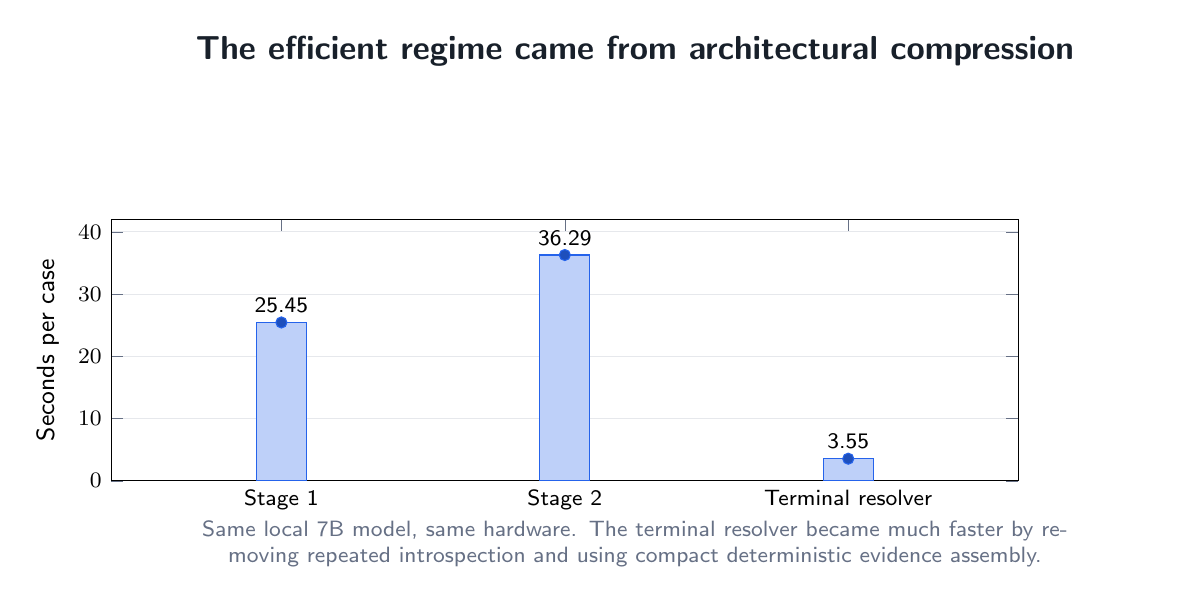
\begin{tikzpicture}
\node[title] at (7.4,6.0) {The efficient regime came from architectural compression};
\begin{axis}[
 at={(0.75cm,0.55cm)},anchor=south west,
 width=13.1cm,height=4.9cm,
 ymin=0,ymax=42,xmin=0.4,xmax=3.6,
 xtick={1,2,3},xticklabels={Stage 1,Stage 2,Terminal resolver},
 ylabel={Seconds per case},ymajorgrids=true,grid style={draw=linegray!45},
 tick label style={font=\sffamily\footnotesize},label style={font=\sffamily\small}
]
\addplot+[ybar,bar width=18pt,fill=blue!30,draw=blue] coordinates {(1,25.45)(2,36.29)(3,3.55)};
\node[font=\sffamily\footnotesize,anchor=south] at (axis cs:1,25.45) {25.45};
\node[font=\sffamily\footnotesize,anchor=south] at (axis cs:2,36.29) {36.29};
\node[font=\sffamily\footnotesize,anchor=south] at (axis cs:3,3.55) {3.55};
\end{axis}
\node[label, text width=135mm] at (7.4,-0.25) {Same local 7B model, same hardware. The terminal resolver became much faster by removing repeated introspection and using compact deterministic evidence assembly.};
\end{tikzpicture}
\end{document}
